%%%%%%%%%%%%%%%%%%%%%%%%%%%%%%
%%  Design pattern creazionali
%%%%%%%%%%%%%%%%%%%%%%%%%%%%%%

\subsection{Dependency injection}

\begin{figure}[H] \label{fig:injector}
	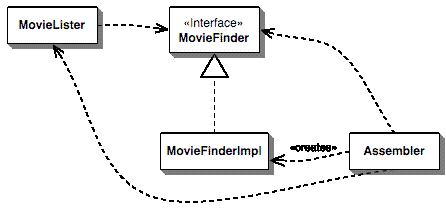
\includegraphics[scale=0.8]{img/injector.png}
	\caption{Dependency Injection.}
\end{figure}

\subsubsection{Scopo} Permette di disaccoppiare il comportamento di una componente dalla risoluzione delle sue dipendenze, semplificando perciò lo sviluppo di un software di grandi dimensioni e allo stesso tempo migliorandone la testabilità.

\subsubsection{Motivazione} Grazie a questo pattern è possibile separare la responsabilità di uso e creazione di un oggetto. Il componente dipendente dovrà solo sapere come usare un servizio richiesto, mentre il compito di creare ed iniettare quest'ultimo spetta ad un injector. Questo permette al componente dipendente di essere altamente configurabile in quanto è fisso solo il suo comportamento.

\subsubsection{Struttura} Sono coinvolti 3 componenti nella dependency injection:
\begin{enumerate}
	\item gli oggetti servizi(ossia un qualsiasi oggetto che potrebbe essere usato);
	\item l'oggetto dipendente da questi servizi;
	\item un injector responsabile di creare ed iniettare i servizi.
\end{enumerate}

\subsubsection{Applicabilità} È possibile applicare il pattern in tre modi differenti:
\begin{itemize}
	\item \textbf{setter injection:} la dipendenza viene iniettata tramite dei metodi setter del component dipendente;
	\item \textbf{costruction injection:} la dipendenza viene iniettata tramite un paramento del costruttore;
	\item \textbf{interface injection:} l'iniezione viene eseguita attraverso l'interfaccia che fornirà un setter a chiunque la implementa.
\end{itemize}

\subsection{Command}

\begin{figure}[H] \label{fig:command}
	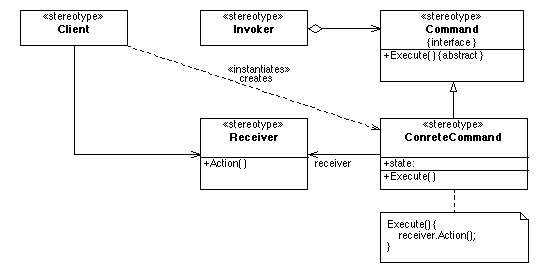
\includegraphics[scale=0.6]{img/command.png}
	\caption{Command.}
\end{figure}

\subsubsection{Scopo} Permette di isolare la porzione di codice che effettua un'azione dal codice che ne richiede l'esecuzione. Tale azione è incapsulata nell'oggetto Command.

\subsubsection{Struttura} Sono coinvolti i seguenti componenti:
\begin{enumerate}
	\item Client: colui che richiede il comando  ed imposta il Receiver;
	\item Invoker: colui che effettua l'invocazione del comando;
	\item Command: interfaccia generica per l'esecuzione del comando;
	\item ConcreteCommand: implementazione del comando che consente di collegare l'invoker con il Receiver;
	\item Receiver: colui che riceve il comando e sa come eseguirlo.
\end{enumerate}

\subsubsection{Applicabilità} È possibile applicare il pattern per:
\begin{itemize}
	\item parametrizzare gli oggetti sull'azione da eseguire;
	\item specificare,accodare ed eseguire richieste molteplici volte;
	\item supportare operazioni di Undo e Redo;
	\item supportare la transazione: un comando equivale ad un'operazione atomica.
\end{itemize}

\subsection{Factory}

\begin{figure}[H] \label{fig:factory}
	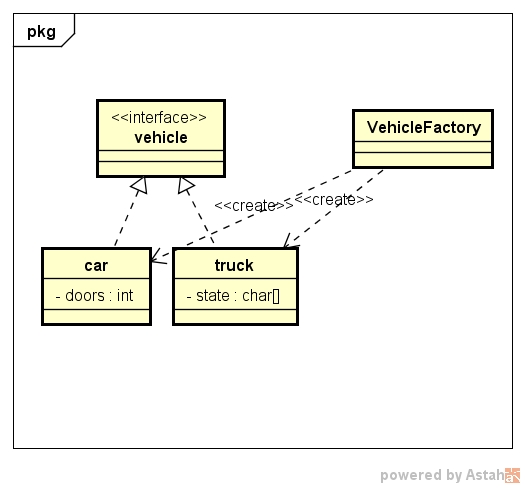
\includegraphics[scale=0.8]{img/factory2.png}
	\caption{Factory.}
\end{figure}

\subsubsection{Scopo} Indirizza il problema della creazione di oggetti senza specificarne la classe esatta fornendo un'interfaccia per creare l'oggetto, ma lascia che le sottoclassidecidano quale oggetto istanziare.

\subsubsection{Struttura} Sono coinvolti i seguenti componenti:
\begin{enumerate}
	\item Creator (VeichleFactory): dichiara la Factory che avrà il compito di ritornare l'oggetto appropriato;
	\item Product (Vehicle): definisce l'interfaccia dell'oggetto che deve essere creato dalla Factory;
	\item ConcreteProduct (Truck,Car): implementa l'oggetto in base ai metodi  definiti dall'interfaccia Product.
\end{enumerate}

\subsubsection{Applicabilità} È possibile applicare il pattern quando:
\begin{itemize}
	\item la creazione di un oggetto preclude il suo riuso senza una duplicazione di codice;
	\item la creazione di un oggetto richide l'accesso ad informazioni o risorse che non dovrebbero essere contenute nella classe di composizione;
	\item la gestione del ciclo di vita degli oggetti gestiti deve essere centralizzata in modo da assicurare un comportamento coerente all'interno dell'applicazione.
\end{itemize}

\subsection{Observer}

\begin{figure}[H] \label{fig:observer}
	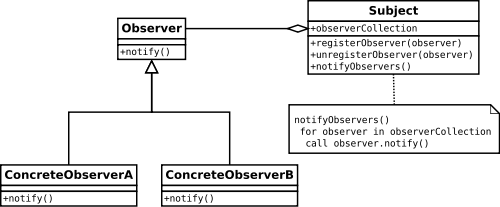
\includegraphics[scale=0.6]{img/observer.png}
	\caption{Observer.}
\end{figure}

\subsubsection{Scopo} Questo pattern viene utilizzato quando si vuole realizzare una dipendenza uno-a-molti in cui il cambiamento di stato di un soggetto venga notiifcato a tutui i soggetti che si sono mostrati interessati.

\subsubsection{Struttura} Sono coinvolti i seguenti componenti:
\begin{enumerate}
	\item Subject: espone l’interfaccia che consente agli osservatori di iscriversi e cancellarsi mantenendi una reference a tutti gli osservatori iscritti;
	\item Observer: espone l’interfaccia che consente di aggiornare gli osservatori in caso di cambio di stato del soggetto osservato;
	\item ConcreteSubject: mantiene lo stato del soggetto osservato e notifica gli osservatori in caso di un cambio di stato;
	\item ConcreteObserver: implementa l’interfaccia dell’Observer definendo il comportamento in caso di cambio di stato del soggetto osservato.
\end{enumerate}

\subsubsection{Applicabilità} È possibile applicare il pattern quando:
\begin{itemize}
	\item in un problema ci sono due aspetti tra loro dipendenti, che possono essere rappresentati come classi che possono essere usati indipendentemente tra loro;
	\item quando il cambiamento di un oggetto provoca un cambiamento in un altro oggetto;
	\item quando un oggetto ha la necessità di comunicare con altri oggetti, senza fare assunzioni sugli altri oggetti.
\end{itemize}
